\section{Data Analysis and Preprocessing}

Our dataset, MIT-BIH Arrhythmia Database, consists of ECG recordings from 47 patients, which includes a total of approximately 30,456,000 ECG signals. The database also provides reference annotations for each beat, totaling around 110,000 annotations.

The dataset comprises ECG data and annotation data, which throws out the difficulty in labeling heart rates with according annotations. That is to say, the Heart Rate Dataset has two columns: timestamp (sampled at 360HZ) and heart beat voltage at such timestamp, while the Annotation Dataset has columns for each heartbeat: the timestamp and the corresponding annotation. To label the heart rate, the first step is to segment heart rate signal into individual heart beat, and label every heart beat with N (normal heart beat) or not N (see \cite{arrhythmia_types}). 

\nocite{physionet}
\nocite{goldberger2000physiobank}

Although algorithms like the bandpass filter can be used to extract heartbeats from ECG waveforms, relying solely on this method may not be sufficient. This is because some heartbeats may fall outside the limitations of the algorithm, leading to inaccuracies in heartbeat detection. However, by utilizing the full annotation data for each heartbeat, we can accurately segment each heartbeat and ensure that no heartbeats are missed or misidentified. The approach we took is to normalize and resample heart rate onto annotations, so that we generate a series of heart beats, each with 128 coordinates, and we can assign classes to every heart beat.
\begin{center}
    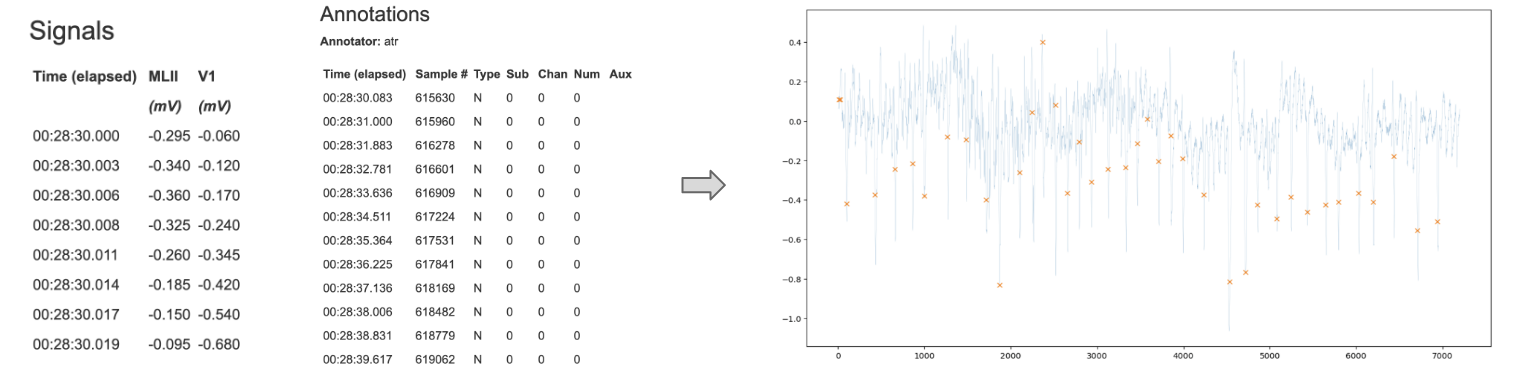
\includegraphics[width=\textwidth]{latex-images/Sub-figures_Example/feature-engineering-1.png}
\end{center}

\begin{center}
    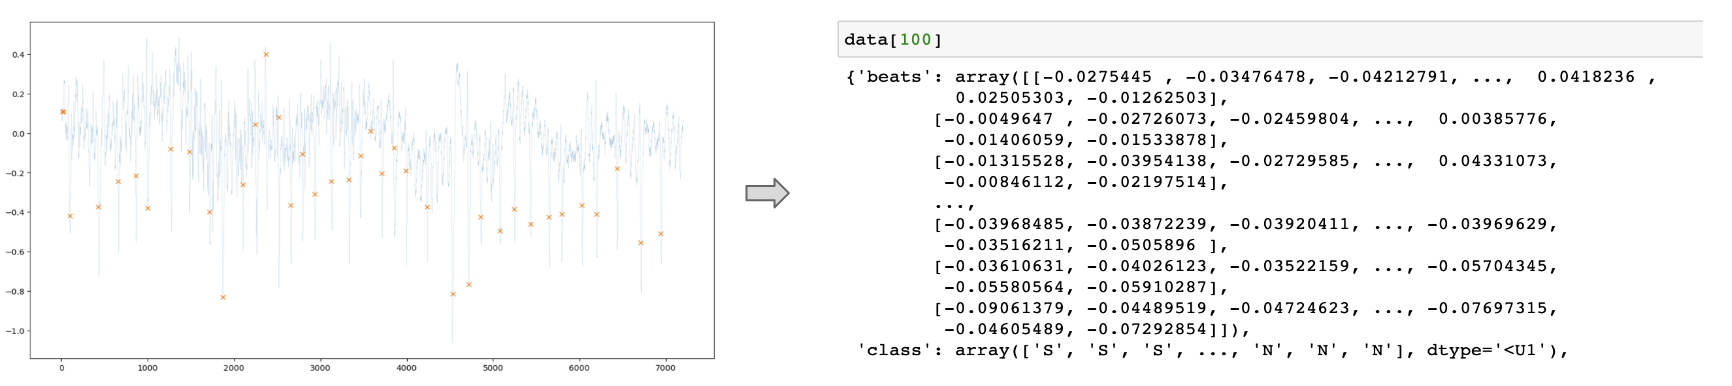
\includegraphics[width=\textwidth]{latex-images/Sub-figures_Example/feature-engineering-2.png}
\end{center}

\nocite{Arrhythmia_Monitoring_System}
